%!TEX root = ../talk.tex

\section{TensorFlow}\label{sec:TF}

%%%
\subsection{Computational graph}
%%%

\begin{frame}[fragile]
  \MyLogo
  \frametitle{Computational graph}  
TensorFlow computations are expressed as stateful dataflow graphs.
\begin{itemize}
\item each node corresponds to an operation (eg tensor, add, sub etc)
\item each edge corresponds to tensor flowing direction
\end{itemize}
%  
\begin{columns}
\column{.57\textwidth}
\begin{lstlisting}[language=python]
import tensorflow as tf

graph = tf.Graph()

with graph.as_default():
	with tf.name_scope('input_var'):
		a = tf.Variable(tf.random_uniform([1, 10], -1.0, 1.0))
		tf.summary.histogram('a', a)
		b = tf.Variable(tf.random_uniform([1, 10], -1.0, 1.0))
		tf.summary.histogram('b', b)
	with tf.name_scope('result'):
		c = tf.multiply(a, b)
		tf.summary.histogram('c', c)
	
	merged = tf.summary.merge_all()
	writer = tf.summary.FileWriter('/home/fan/board', graph)

with tf.Session(graph=graph) as sess:
	tf.global_variables_initializer().run()
	print sess.run([a, b, c])
	writer.add_summary(merged.eval())

writer.close()

\end{lstlisting}
%
\column{.48\textwidth}
%
\begin{figure}[htbp] 
   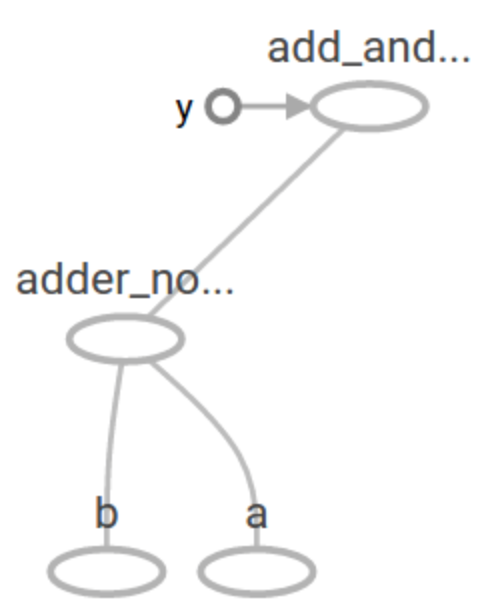
\includegraphics[height=1.5in]{figures/compgraph.png} 
\caption{Computaion graph}
\end{figure}
\end{columns}
\end{frame}

%%%
\subsection{Programming interface}
%%%

\begin{frame}
  \MyLogo
  \frametitle{Programming interface}
  In this section we provide a discussion of the computational graph architecture underlying the TensorFlow software library.
  
  \begin{itemize}
	  	\item Graph: In TensorFlow, machine learning algorithms are represented as computational graph. A computational or dataflow graph is a form of directed graph where vertices or nodes describe operations, while edges represent data flowing between these operations.
	  	
	  	\item Operation: An opreation may represent a mathematical equation, a variable or constant, a control flow directive, a file I/O operation or even a network communication port.
	  	
	  	\item Tensor: A tensor is a multi-dimensional collection of homogeneous values with a fixed, static type.
	  	
	  	\item Variable: Variables can be described as persistent, mutable handles to in-memory buffers storing tensors.
	  	
	  	\item Session: In TensorFlow the execution of operations and evaluation of tensors may only be preformed in a special environment called session.
  \end{itemize}

\end{frame}

%%%
\subsection{Visualization}
%%%

\begin{frame}
  \MyLogo
  \frametitle{Visualization: TensorBoard}  

\begin{columns}
\column{.48\textwidth}  
\scriptsize{
Computation graphs are powerful but complicated
\begin{itemize}
\item  thousands of nodes or more 
\item  network is deep
\item  graph visualization tool TensorBoard is helpful
\end{itemize}
}
%
\column{.5\textwidth}
\begin{figure}[htbp] 
   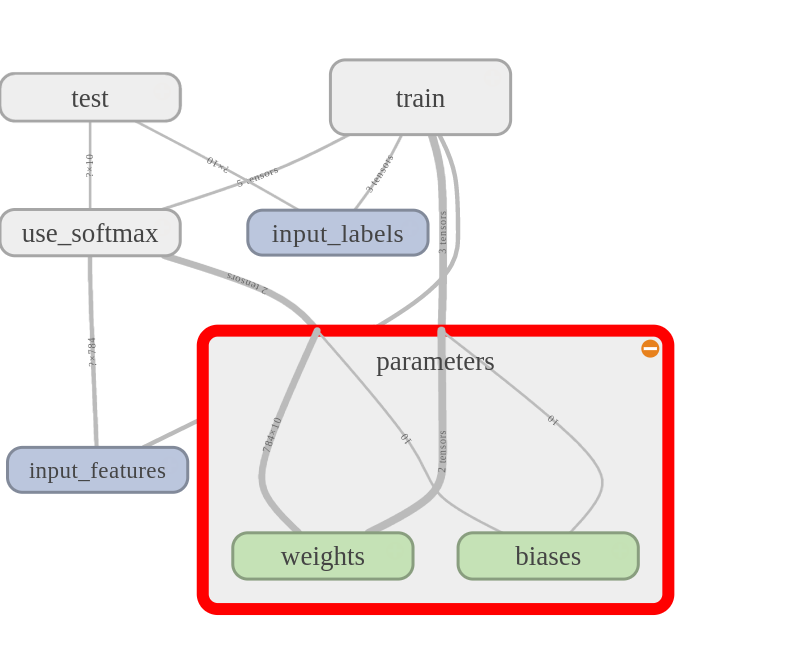
\includegraphics[height=2.5in]{figures/graphvisualization.png} 
\caption{Graph Visualization}
\end{figure}
\end{columns}

\end{frame}

%%%
\subsection{Some examples}
%%%

\begin{frame}[fragile]
  \MyLogo
  \frametitle{Example 1: SoftMax}  
 
\scriptsize{
\begin{lstlisting}[language=python]
import tensorflow as tf

# Import the training data (MNIST)
import tf.examples.tutorials.mnist.input_data as input_data

# Possibly download and extract the MNIST data set
# Retrieve the labels as one-hot-encoded vectors
mnist = input_data.read_data_sets("MNIST_data/", one_hot=True)

# Create a new graph
graph = tf.Graph()

# Set our graph as the one to add nodes to
with graph.as_default():
	# Placeholder for input variables (None = variable dimension)
	x = tf.placeholder("float", shape=[None, 784])
	# Placeholder for labels
	y_ = tf.placeholder("float", shape=[None, 10])
	
	# Weights and bias
	W = tf.Variable(tf.zeros([784, 10]))
	b = tf.Variable(tf.zeros([10])) 
\end{lstlisting}
}
\end{frame}

\begin{frame}[fragile]
  \MyLogo
  \frametitle{Example 1:SoftMax}  
\scriptsize{
\begin{lstlisting}[language=python]
	# Apply softmax regression model
	y = tf.nn.softmax(tf.matmul(x, W) + b)
	
	# Compute the cross entropy of y_ and y
	entropy = -tf.reduce_sum(y_*tf.log(y))
	# Create a gradient-descent optimizer
	train_step = 
		tf.train.GradientDescentOptimizer(0.01).minimize(entropy)
		
	# Find the indices where the predictions were correct
	correct_prediction = tf.equal(tf.argmax(y,1), tf.argmax(y_,1))
	accuracy = tf.reduce_mean(tf.cast(correct_prediction, "float"))

with tf.Session(graph=graph) as session:
	# Initialize all variables
	tf.global_variables_initializer().run()
	
	# Train the model
	for step in range(1000):
		batch_x, batch_y = mnist.train.next_batch(100)
		train_step.run(feed_dict={x: batch_x, y_: batch_y})
	# Print the accuracy using the model
	print accuracy.run(feed_dict={x: mnist.test.images, 
								y_:mnist.test.labels})
\end{lstlisting}
}

%\end{tabular}

%\end{center}
%\label{default}
%\end{table}%
\end{frame}